\cleardoublepage

\chapter{Introduction}
\label{chapter1}
\section{Motivation}
Increased life expectancy and sedentary lifestyles have boosted the appearance of chronic lifestyle-associated diseases. This has repercussions both at patient-level, with a significant loss of life quality, and at greater levels, increasing the pressure over national health systems.

Diabetes, which already affects one in ten adults, is undoubtedly one of the more damaging and harder to control. 783 million of people are projected to live with diabetes by 2045 and the cost of treating the disease has more than triplicated in the last 15 years \cite{diabetesatlas}.

A common complication of diabetes is diabetic retinopathy (DR) (around 40\% to 45\% of patients with diabetes have some stage of the disease\cite{drPatients}), caused by the vascular damages provoked by a persistently high blood sugar level. DR is already the main cause of new cases of blindness in adults and has a cost of over 500 million USD just in the US. Early detection is key, as the most evident signs show up when the disease is already too advanced to be effectively treated. 

The most common way to detect the disease is \textit{ophthalmoscopy}. This technique consists in the dilation of the pupil to photograph the \textit{fundus} of the retina (which includes the central and peripheral retina, the optic disc and the macula) using a specialized camera. The diagnosis of the disease is then carried by a professional clinician, who will carefully examine the photographs and grade the degree of diabetic retinopathy affectation in each eye in a scale from 0 to 4. The quality of the final images depends on the equipment used and the ability of the professional. \Cref{fig:disease_summary} shows some examples of ophthalmoscopy images of different patients from the EyePACS dataset\cite{cuadros2009eyepacs}, labelled by the grade of the disease. The images serve as an example on how remarkably similar healthy and severely ill eyes may appear to the untrained eye.

\begin{figure}[tb]
     \begin{subfigure}[b]{0.3\textwidth}
         \centering
         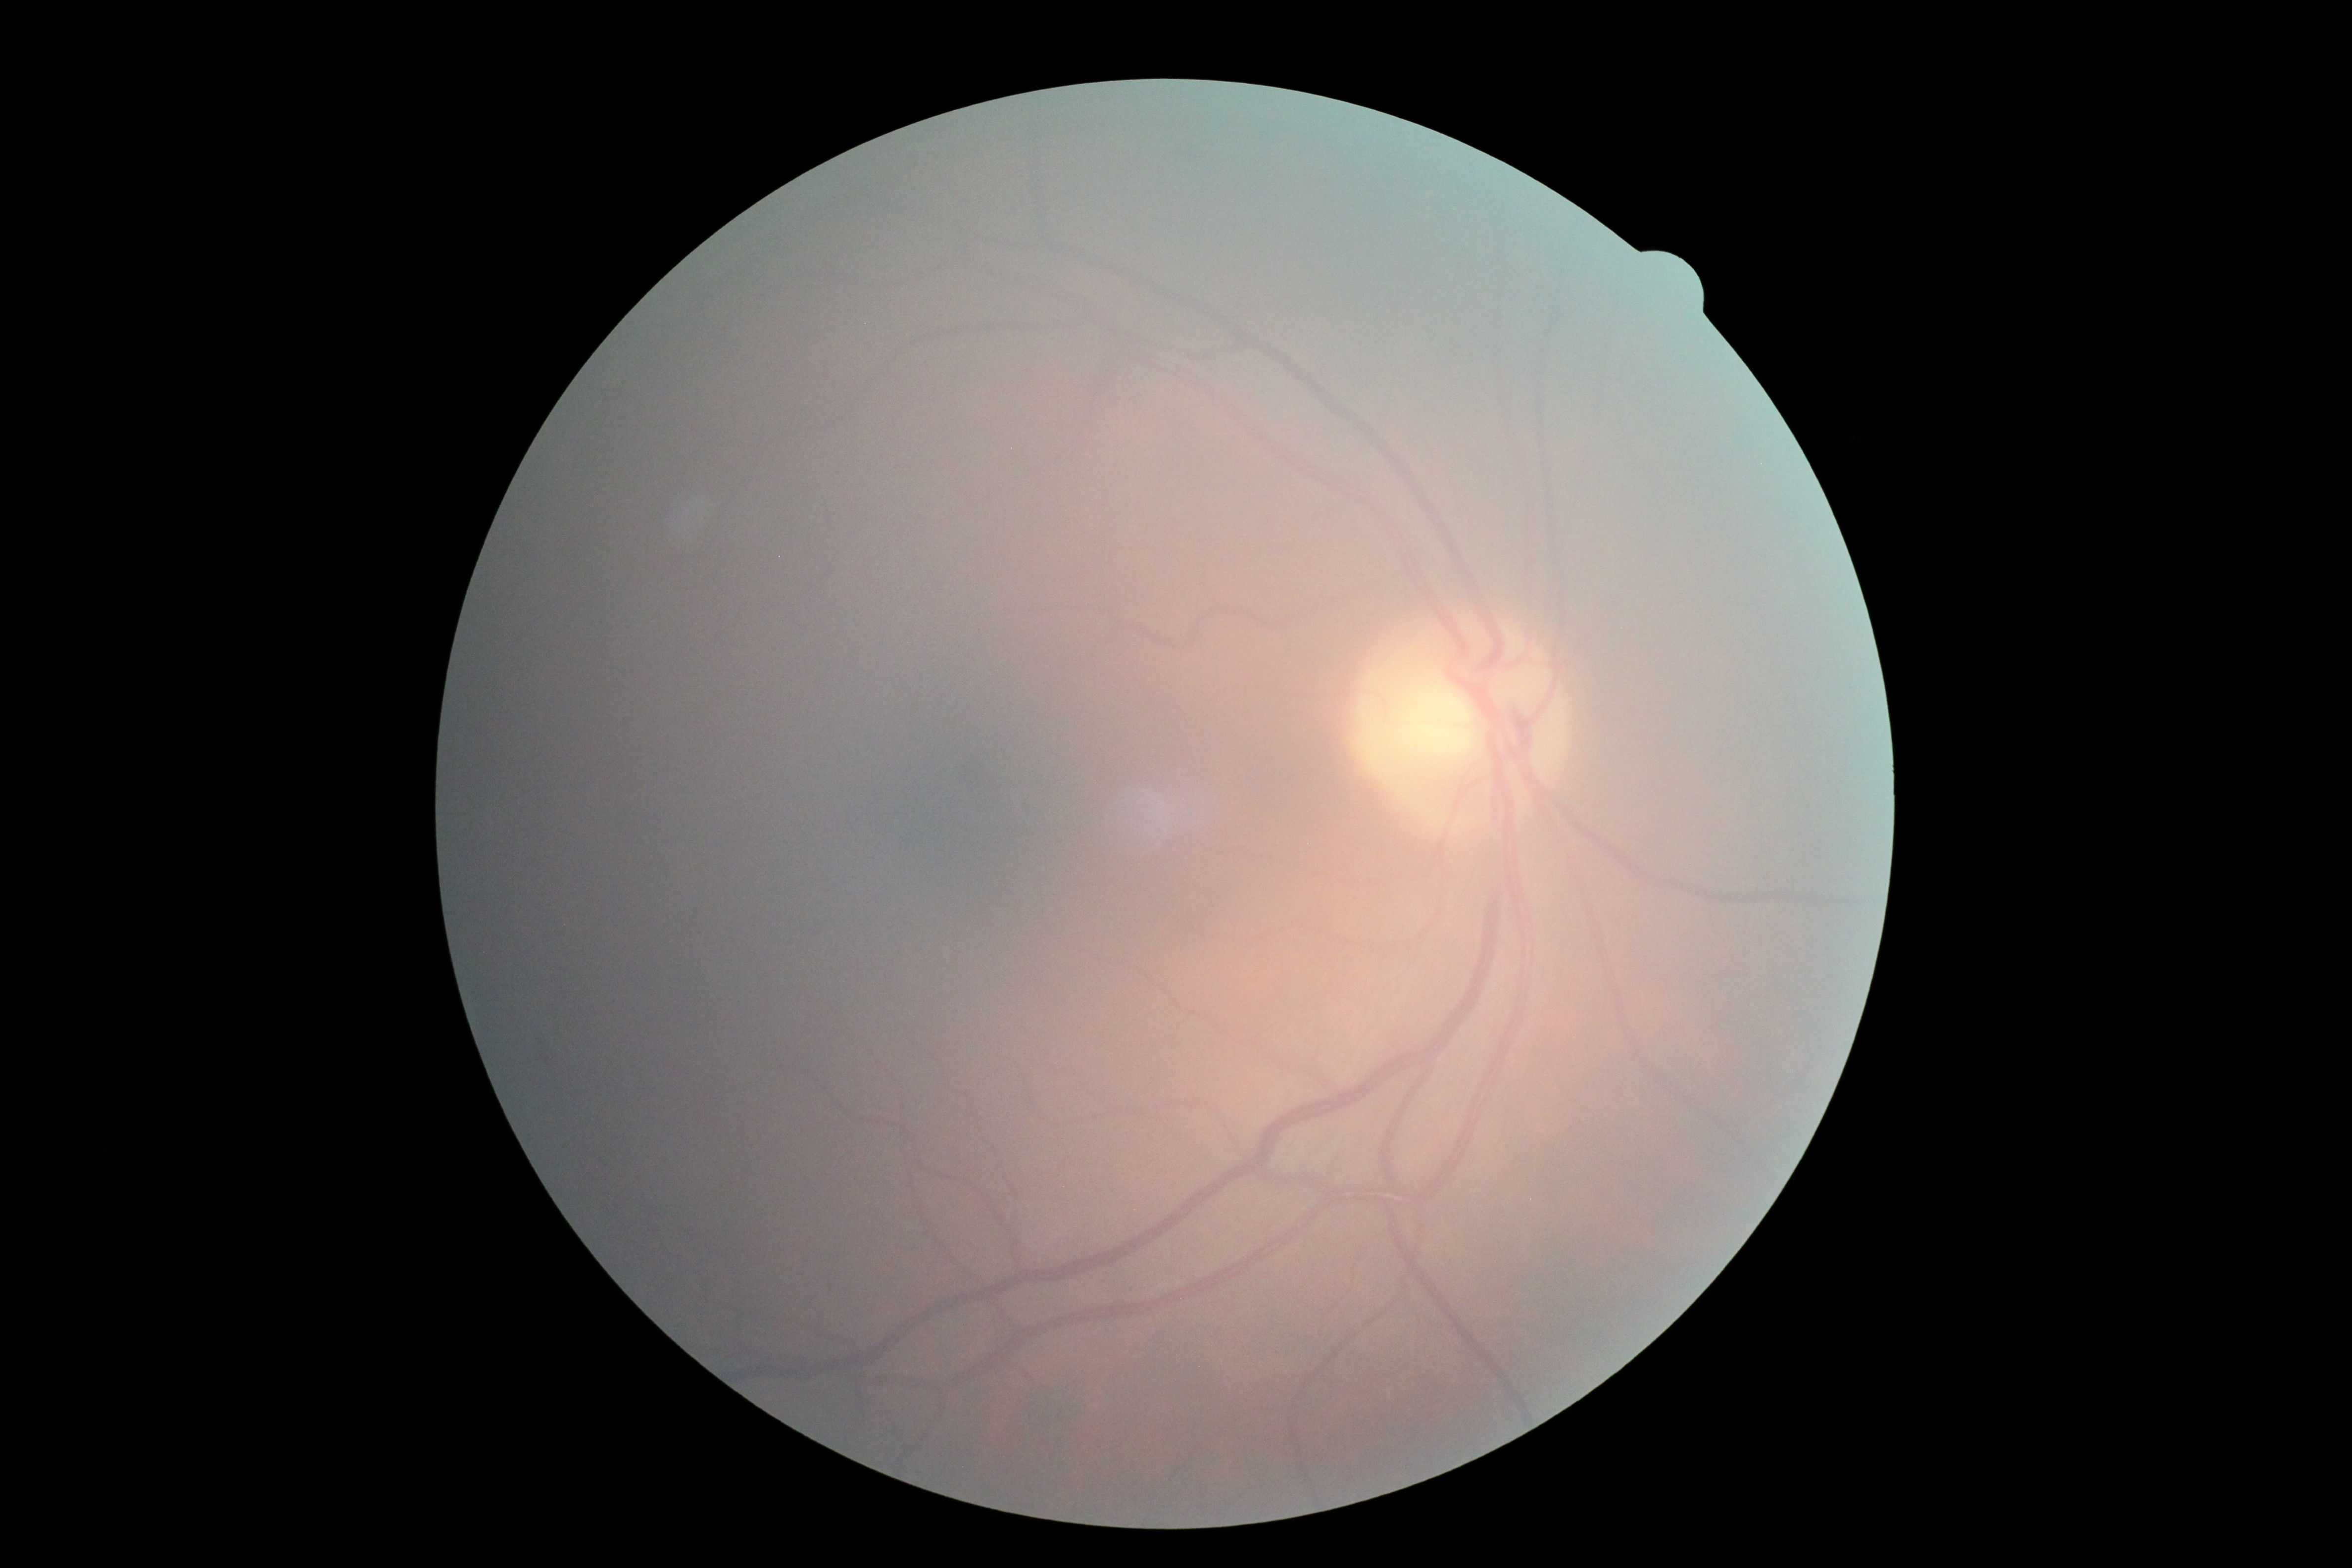
\includegraphics[width=\textwidth, height=\textwidth]{figures/chapter4/Dataset/noDR/75_right.jpeg}
         \caption{Grade 0}
    \end{subfigure}
     \hfill
         \begin{subfigure}[b]{0.3\textwidth}
        \centering
        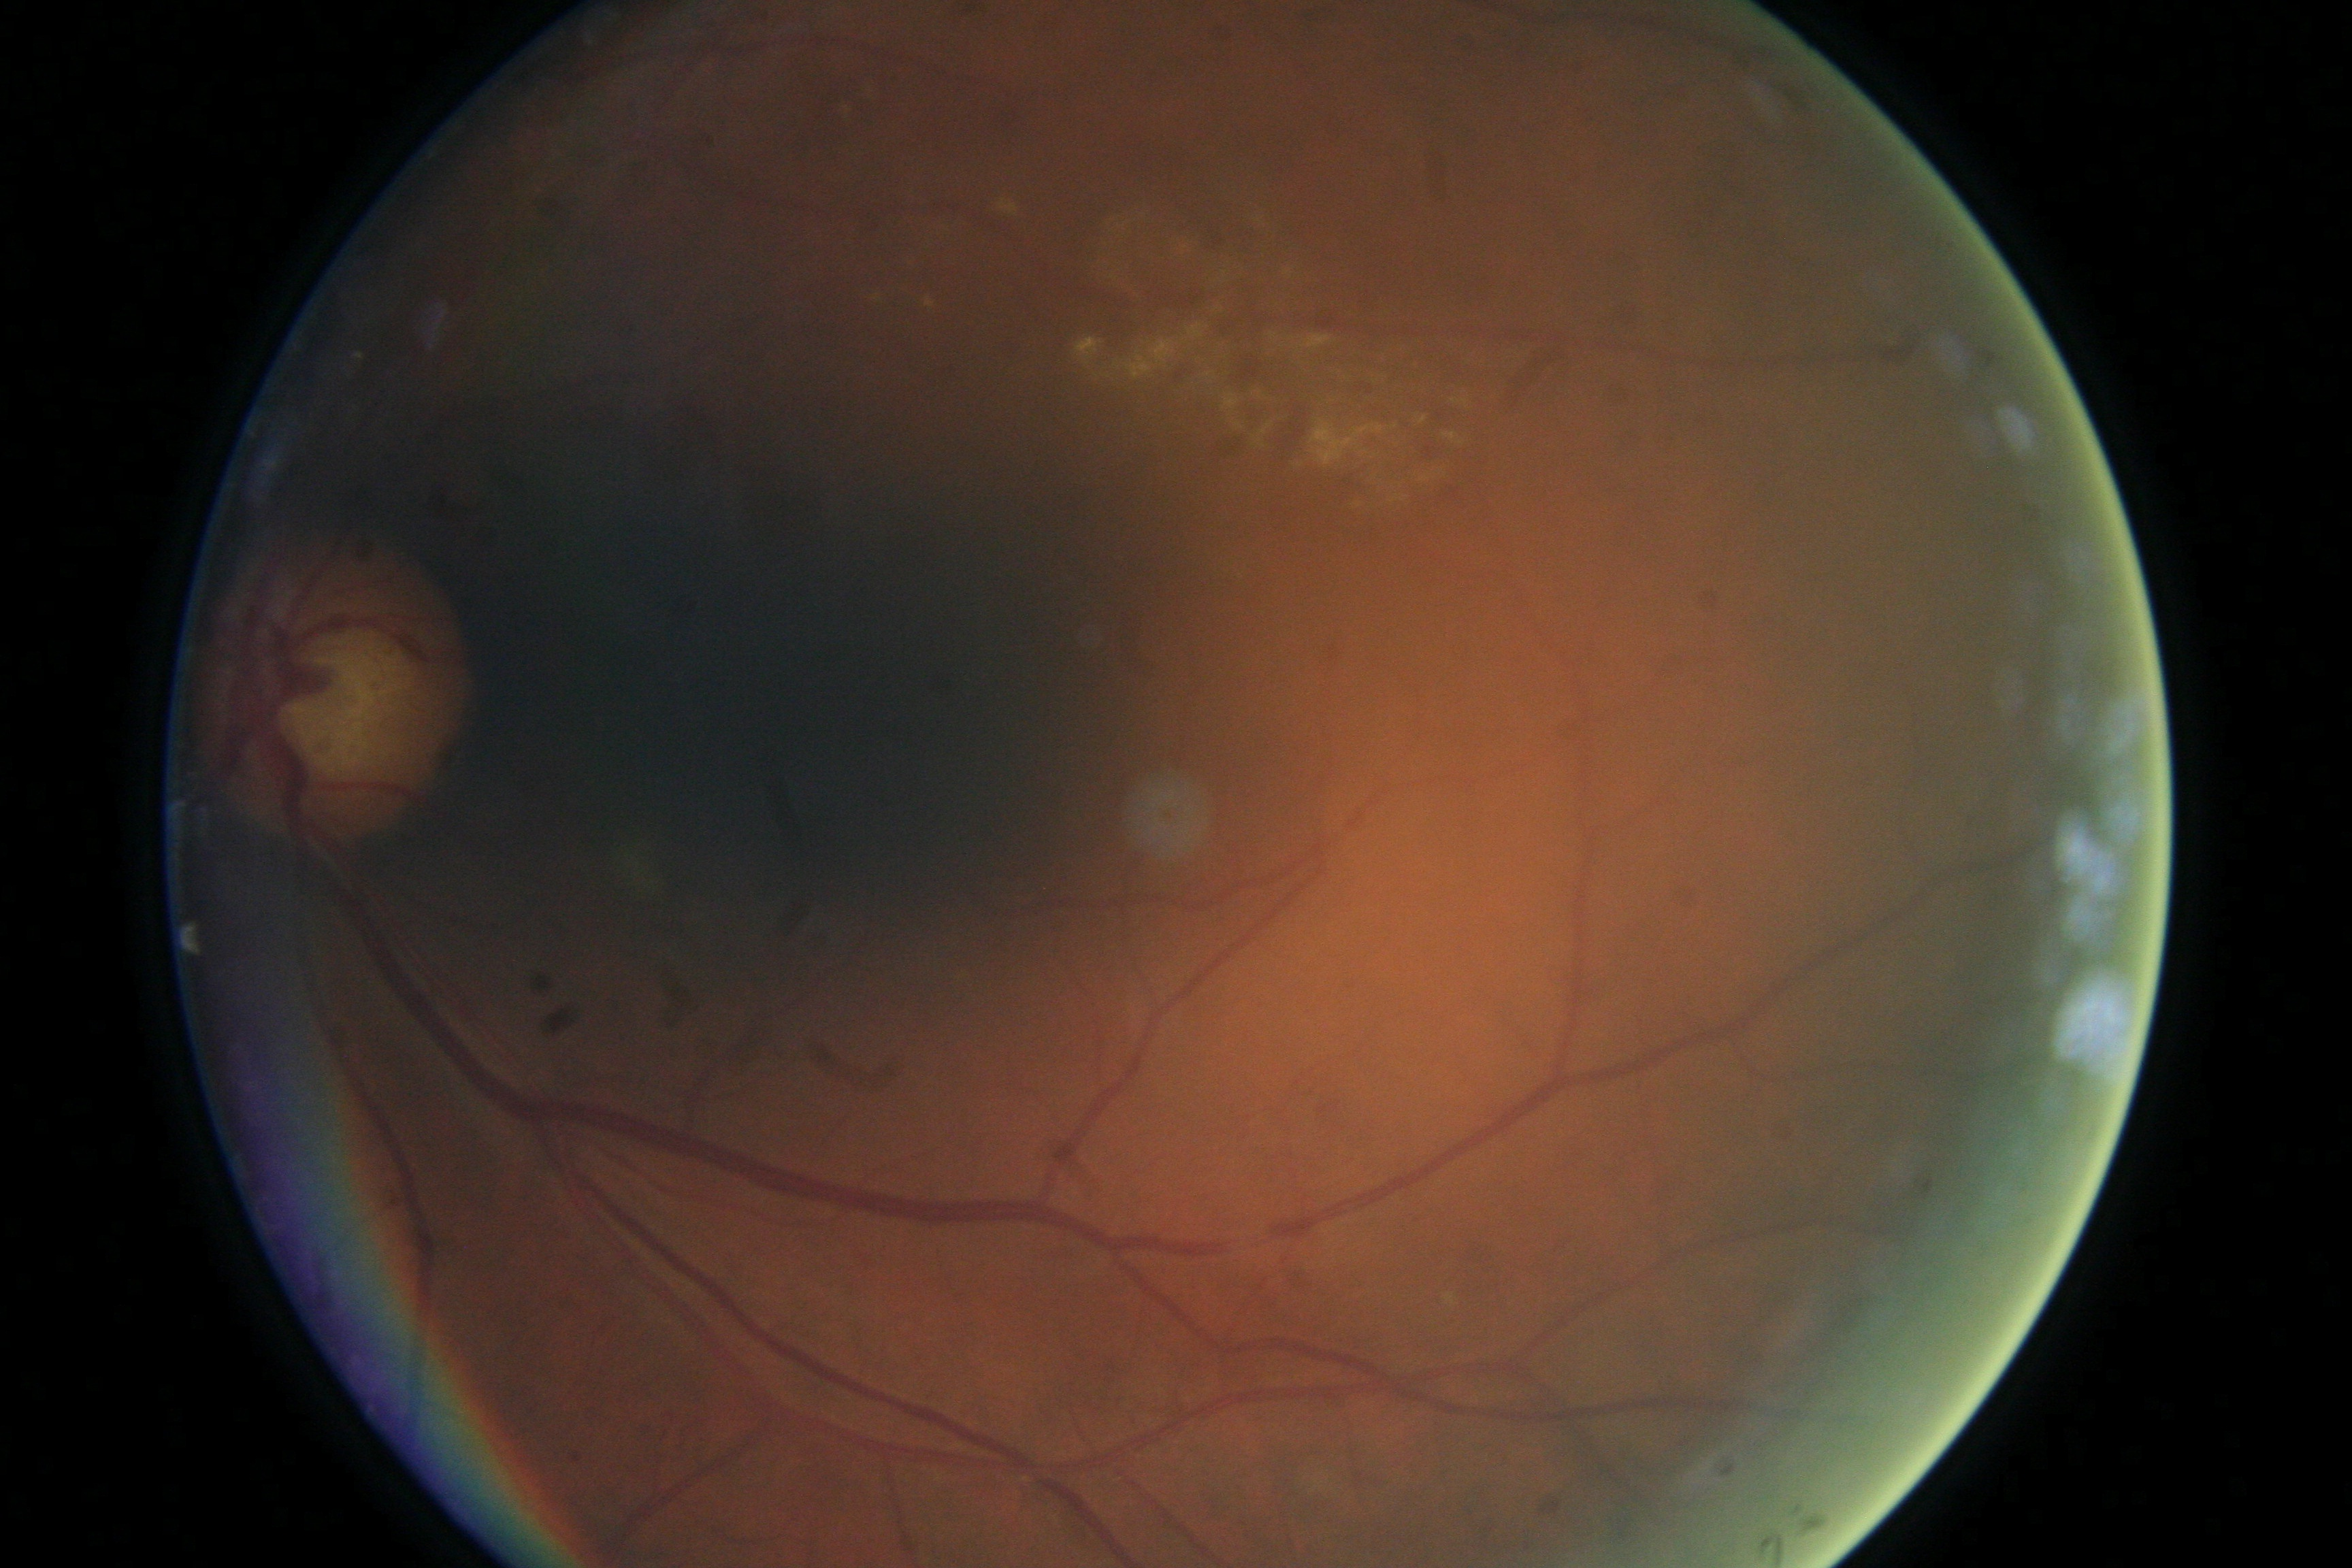
\includegraphics[width=\textwidth, height=\textwidth]{figures/chapter4/Dataset/moderate/54_right.jpeg}
        \caption{Grade 2}
    \end{subfigure}
    \hfill
     \begin{subfigure}[b]{0.3\textwidth}
        \centering
        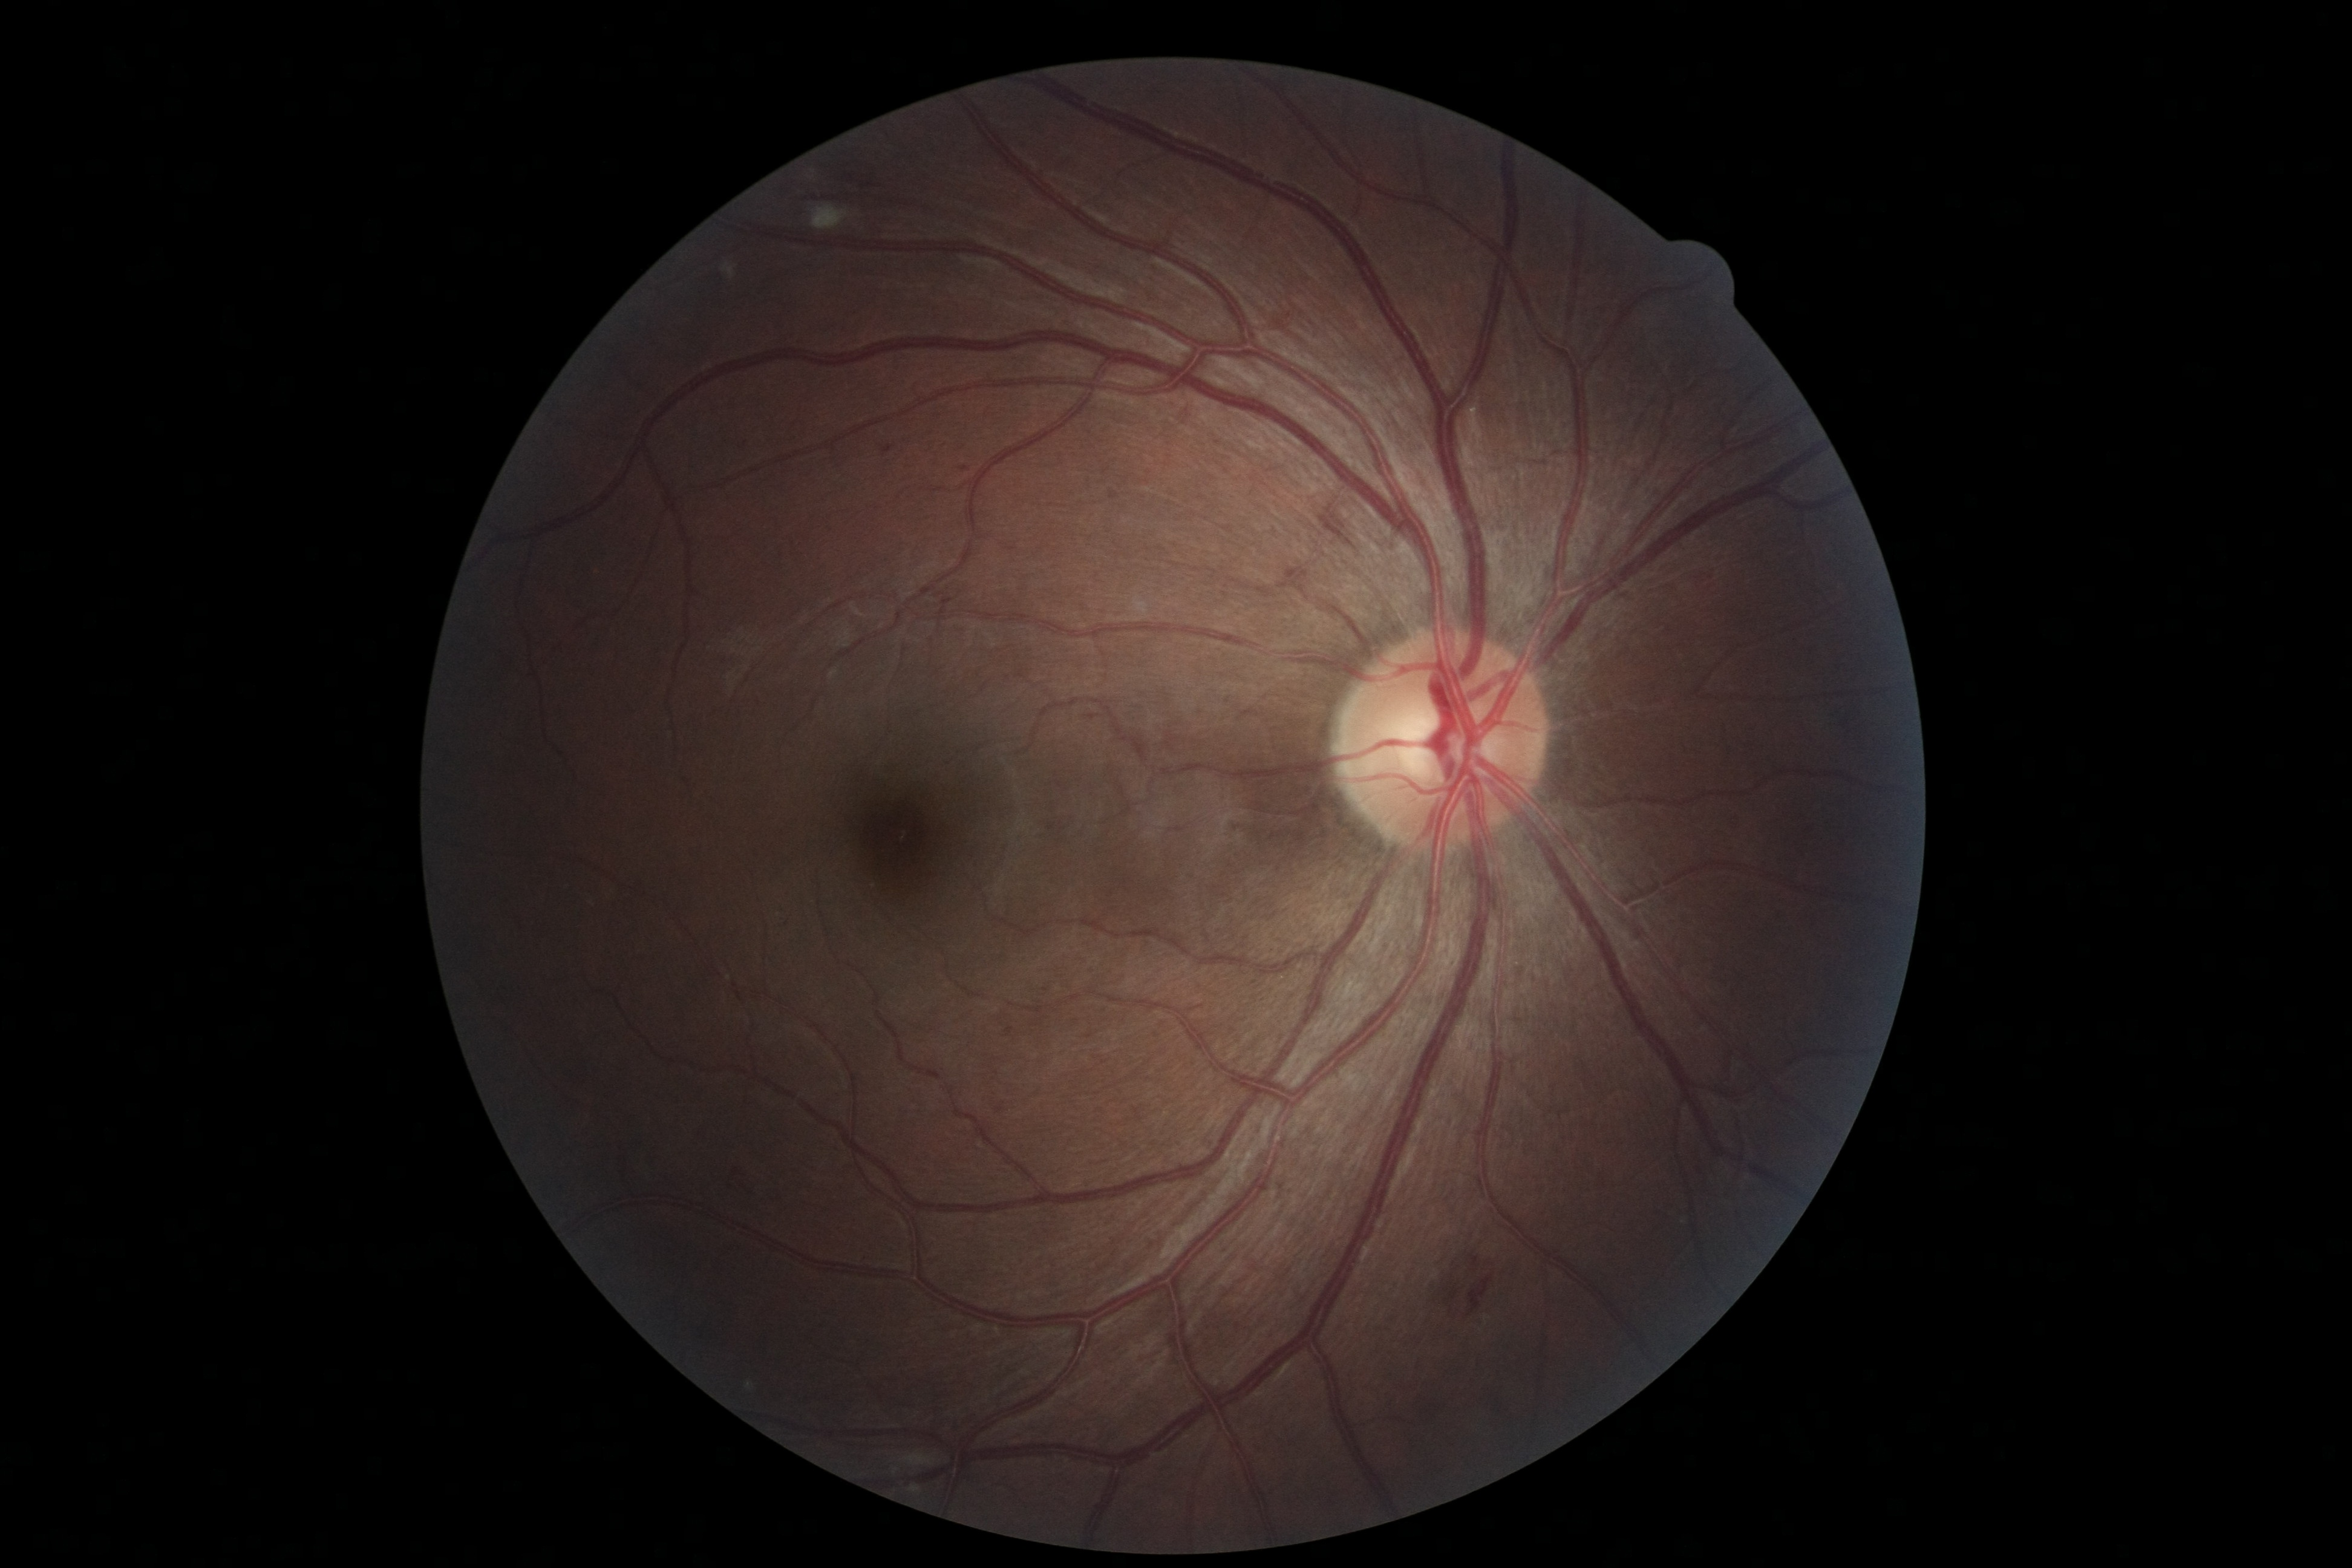
\includegraphics[width=\textwidth, height=\textwidth]{figures/chapter4/Dataset/proliferative/352_right.jpeg}
        \caption{Grade 4}
    \end{subfigure}
    \caption{Example of images of different classes. Note the different color, brightness, and scale of each image.}
    \label{fig:disease_summary}
\end{figure}

The process of diagnosis presents some difficulties. In first place, the aspect of the image is heavily dependent on the equipment used, and it is common for fundus images to show some kind of noise, in the shape of over or underexposure, blur… In second place, some signs of the disease (as microaneurysm or blood vessel narrowing) are quite small and hard to detect even by a trained professional. These problems, among others, explain why studies have found that different clinicians agree on the grading of DR of an eye only on 69\% of the cases and may differ by two levels or more in around 9\% of the cases \cite{gangaputra2013comparison}. 

Diagnosing is also a time-consuming process and results are usually submitted one or two days after examination \cite{diabeticretinopathydetection}, which can lead to loss of follow-up with the patient, miscommunication and delayed treatment.

There are additional problems surrounding diagnosis. Specialized equipment is expensive and training a professional to take the photographs and interpret the images requires years. Generic training in ophthalmology (which usually requires more than ten years) is not enough, as previous studies have found that retina expert without specific DR training are less consistent at grading DR and show greater inter-grader variability \cite{grzybowski2022variability}.

The expertise and equipment are usually lacking in those areas more affected by the disease, as 3 out of 4 cases of diabetes are diagnosed in low or middle-income countries.

The necessity for an automated method to screen for DR was detected years ago, as it could drastically reduce the necessary time for diagnosis, allowing earlier treatment and better patient outcome \cite{diabeticretinopathydetection}. Ideally, such a method should not only be able to accurately grade the disease but also to identify and segment the regions with diagnostic significance, so a trained professional can interpret its results.

Since then, significant progress has been made in the area. The first automated methods tried to replicate clinical guidelines, usually looking for morphological changes on blood vessels and the presence of lesions, especially microaneurysms and hemorrhages \cite{verma2011detection}. While this was usually enough to achieve a good accuracy, these methods were unable to recognize global phenomena and its design required significant domain knowledge. As most techniques were highly tailored for diabetic retinopathy detection, advances in other areas (as the diagnosis of other similar diseases) could not be reused for DR detection.

The introduction of deep learning models for DR grading has provoked a breakthrough in the field. These models do not try to replicate the process followed by a clinician and require little to no domain knowledge. Indeed, research has shown that a wide spectrum of general purpose deep learning models can be repurposed to grade DR with excellent precision. Deep learning based models have displaced previous alternatives and are the backbone of contemporary techniques for DR grading \cite{gupta2018diabetic}. 

There are, however, various problems with deep learning models. Training these models requires significant computational resources and is out of reach for organizations without dedicated hardware. Deep learning models behave as a black box and interpreting its results can be very challenging, hindering its applicability in a clinical setting.

The objective of this work is to design and implement a deep learning model for DR grading based in state-of-the-art results that can perform training and inference under strict computational requirements and achieve solid performance, while offering ample interpretability capabilities.

We believe our work covers a research gap, as the topic of DR grading using \textit{deep learning} models under strict computational requirements has not been sufficiently studied. 

This is a regrettable omission, as automated techniques are especially useful in contexts with limited resources, where computing power is highly limited. While we explore the viability of training a model in a medium-grade customer PC, we believe it can be expanded, so inference can be carried in mobiles.

In order to contextualize our work, we introduce a comprehensive review on \textit{deep learning} from first principles (focusing on computer vision techniques) and a survey on the evolution of DR grading using computer automated techniques.

\section{Objectives}
Computer vision is dominated by two families of models: \textit{convolutional neural networks} (CNNs) and the much more recent \textit{vision transformers}. While the latter show unparalleled scalability, the former achieve the best parameter/accuracy ratio, which makes them the first option of choice when working under strict computational limits. 

We will explore various standard architectures of CNNs and select one able to offer the required compromise between accuracy and efficiency. We will also look into some techniques to reduce computational costs at training, like \textit{transfer learning}. 

Once the model has been trained, it will be necessary to assess its performance. This includes comparing it with other, previous results in the field as well as evaluating some of its properties, as \textit{calibration}.

While CNNs are notoriously hard to interpret, a wide variety of techniques to visualize their performance have been devised. We want to adapt some of these techniques to our model and use it to explain its performance.

While we have focused our attention to CNNs, we will provide a revision of both `classical' methods and alternative deep learning architectures in the state-of-the-art review. As a secondary objective, we will explore vision transformers and assess their performance and interpretability properties. 

In summary, the main objectives we will pursue are:
\begin{enumerate}[label=(O\arabic*)]
    \item Identify the state-of-the-art options for computer vision problems and understand their strengths and weaknesses. 
    \item Further our understanding of the disease, its detection and the associated difficulties. Review the field of computer-aided diagnosis, paying special attention to deep learning based approaches.
    \item Find a suitable dataset of retinographies for diabetic retinopathy grading. Ideally, it should be a widely used dataset, so our results are easily comparable to those of previous works. Explore the dataset and preprocess the images if necessary. \label{preprocess}
    \item Create a computationally efficient model (both for inference and learning) based in computational neural networks able to accurately grade the severity levels of DR on fundus images. This comprises the following tasks: \label{firstObj}
    \begin{enumerate}[label=(O\arabic{enumi}.\arabic*)]
        \item Analyze the available deep learning models and identify those better suited for the problem at hand.\label{deepModels}
        \item Choose a model and train it on the dataset. \label{modelChosen}
        \item Evaluate its performance, identifying the more convenient metrics to recognize strengths and weaknesses of the model
    \end{enumerate}
    \item As a stretch goal, we would like to study the necessary extensions of the model to address some lateral tasks: \label{extModel}
    \begin{enumerate}[label=(O\arabic{enumi}.\arabic*)]
        \item Semantic search of retinal images: finding images with a similar diagnostic profile to one given.
        \item Blood vessel or lesion segmentation
    \end{enumerate}
    \item Develop interpretability tools to understand the way the model creates predictions. This entails:
    \begin{enumerate}[label=(O\arabic{enumi}.\arabic*)]
        \item Review the existing tools to interpret deep learning models
        \item Implement some of these techniques, so the behavior of the model can be interpreted by a domain expert.
        \item Assess and compare the performance of these techniques
    \end{enumerate}
    \item Compare the implemented model with a solution based on \textit{vision transformers}, both in terms of accuracy and interpretability. \label{vitvsCNN}
\end{enumerate}

\section{Structure of this document}
The document has been organized, so it can be followed and understood by people with little to no knowledge about deep learning techniques. 

In \Cref{chapter2} we offer an introduction to Deep Learning from first principles, presenting the problem of defining and training neural networks. We recommend the reader to make sure they are comfortable with these concepts before going on as the rest of the presentation will heavily depend on these. We pay special attention to the two deep learning architectures dominating computer vision: convolutional neural networks and vision transformers.

\Cref{chapter3} serves as an introduction to Diabetic Retinopathy disease and computer-aided detection. We carry out a revision of the state-of-the-art techniques for diagnosis and the core ideas behind them.

In \Cref{chapter4} we analyze the dataset of fundus images used and explore how to preprocess the images, so they become adequate for training. As is often the case with clinical images, class distribution is unbalanced, images come from a variety of sources and significant preprocessing is necessary before the images can be effectively used.

In \Cref{chapter5} we review some state-of-the-art CNN architectures and discuss its performance and use cases. We also introduce the convolutional neural network model we used, a customized and fine-tuned EfficientnetV2 model, and the results we obtained, comparing with previous results on the field. 

\Cref{chapter6} explores an interesting lateral application of the CNN embeddings: identifying images with similar diagnostic features. We study the viability of using this technique in clinical practice in two experiments with a professional ophthalmologist.

In \Cref{chapter7} we explore different techniques to interpret and visualize the inner workings of convolutional neural networks. While neural networks are black-box models, visualizations like the \textit{class activation map} can give invaluable insights about the inner workings of the network.

%CAMBIAR
In \Cref{chapter8} we compare the CNN approach to a vision transformer based one. We define, train and evaluate a specialized vision transformer and investigate its interpretability possibilities. 

Finally, we expose our conclusions and evaluate the fulfillment of our objectives. We also indicate some lines of future work, paying especial attention to the obstacles that need to be overcome before a tool like this integrates in clinical practice.

\section{Code}
All the code used for this project has been made public in a GitHub repository, under the MIT license \cite{codeused}. The repository contains instructions on how the repository is structured and how can it be used to reproduce our results. We can also provide the weights of the trained network upon request.

The code for calibrating the model depends on the published code from the paper \textit{On calibration of modern neural networks} \cite{guo2017calibration}, which is used calculates to estimate the calibrating constant. You can use the constant we found, but if you retrain the model in a different dataset you may need to estimate a new constant.

The vision transformer we have trained is an adaptation of the one present in \textit{MIL-VT: Multiple Instance Learning Enhanced Vision Transformer for Fundus Image Classification} \cite{suang2021milvt}. To reproduce the results, you can download the code from the repository the authors have provided and use our training code.